%%%%%%%%%%%%%%%%%%%%%%%%%%%%%%%%%%%%%%%%%%%%%%%%%%%%%%%%%%%%%

\mainmatter%
\setcounter{page}{1}

\lectureseries[\course]{\course}

\auth[\lecAuth]{Lecturer: \lecAuth\\ Scribe: \scribe}
\date{January 12, 2010}

\setaddress%

% the following hack starts the lecture numbering at 1
\setcounter{lecture}{2}
\setcounter{chapter}{2}

\lecture{Behavior Near Equilibria}

\section{Qualitative Behavior Near Equilibria}
This is a continuation of last lecture focusing on \S2.3.1 of Khalil. Looking back at the the phase portraits we can describe some properties of the trajectories of the systems based on the eigenvalues.

\subsection{Case 1}
This case occurs when $\lambda_1<0$ and $\lambda_2<0$. The two lines are the eigenvectors. Assuming $|\lambda_1| > |\lambda_2|$ then the system will start following the eigenvector associated with $\lambda_2$ as $t\to0$ and follow the eigenvector associated with $\lambda_1$ as $t\to\infty$. This is due to the rate of decay of the exponential that solves $\dot{x}=Ax$ or $x=e^{At}$.

\subsection{Case 2}
In oscillatory systems the eigenvalues will have imaginary parts. When $\alpha=0$ we get the mass-spring (no damping) or linear harmonic oscillator behavior. When that happens there is no decay or growth in the trajectories.

\subsection{Case 3}
When $k=0$ the trajectories are straight because the rate of decay of the exponentials is equal since $\lambda_1=\lambda_2$. When $k=1$ the trajectories are parallel with the eigenvector near $t=0$. Multiplicity of the eigenvalues can occur and the exponential describing the system response can contain polynomials such as $e^{t^2}$ and $e^{t^3}$.

\section{Examples of Behavior Near Equilibria}
\begin{example}
\label{ex:03pendulum}
This is Example 2.4 in Khalil and looks at a pendulum with friction. We can use Newton's second law to find the dynamics as
$$ml\ddot{\theta} + kl\dot{\theta} + mg\sin\theta = 0$$
The state space variables are angular position and angular velocity, see Figure~\ref{fig:03pendulum}, where
$$ x_1 = \theta, \qquad x_2 = \dot{\theta}$$
This leads to
\begin{align*}
\dot{x}_1 &= x_2 \\
\dot{x}_2 &= -\tfrac{g}{l}\sin x_1 - \tfrac{k}{m}x_2
\end{align*}
The steps involved in analyzing the system behavior are to find the equilibria, compute the Jacobian and then plot the behavior. The equilibria are at
$$x^{(1)} = \left[\begin{array}{c} 0 \\ 0 \end{array}\right], \qquad x^{(2)} = \left[\begin{array}{c} \pi \\ 0 \end{array}\right]$$
At both equilibria the velocity is zero but the angle differs. The Jacobian can be computed as
$$\frac{\partial{} f}{\partial{} x} = \left[\begin{array}{c c} 0 & 1 \\ -\tfrac{g}{l}\cos x_1 & -\tfrac{k}{m} \end{array}\right]$$
with
$$A_1 = \left[\begin{array}{c c} 0 & 1 \\ -\tfrac{g}{l} & -\tfrac{k}{m} \end{array}\right], \qquad A_2 = \left[\begin{array}{c c} 0 & 1 \\ \tfrac{g}{l} & -\tfrac{k}{m} \end{array}\right]$$
If we let $l=g$, $k=\tfrac{m}{2}$ this leads to a constant $A_1$ and $A_2$. Then the eigenvalues for $A_1$ are
$$\lambda_{1,2} = -0.25\pm{} j0.97$$
and for $A_2$ they are
$$\lambda_1 = -1.28, \qquad \lambda_2 = 0.78$$
From our previous analysis this means that $A_1$ is a stable focus and $A_2$ is a saddle point. Next we look at the eigenvectors to determine orientation. With the left point corresponding to $x^{(1)}$ and the right point to $x^{(2)}$ we can see the phase portrait in Figure~\ref{fig:03multeq}. The two local behaviors, or sets of trajectories, must connect into a global trajectory as seen in Figure~\ref{fig:03globaleq}. The different trajectories are caused by different initial conditions. Note that $x^{(2)}$ corresponds to upright position and $x^{(1)}$ is downward position. That is why the trajectory moves from the right equilibria (top position) to the left equilibria (bottom position) and there is oscillatory behavior around the bottom position.

The natural state space of the system is a cylinder, or the product of the real line for velocity and a circle for position. When the pendulum is swinging around without stopping the trajectory can be thought to be moving around the outside of the cylinder. When friction (damping) stops the pendulum from reaching the top position the trajectory begins to spiral in around a fixed equilibirum point on the cylinder until it stops at the bottom position.
$\lozenge$
\end{example}

\begin{figure}[ht!]
\centering
\includegraphics[width=.5\textwidth]{images/03pendulum}
\caption{Pendulum.}
\label{fig:03pendulum}
\end{figure}

\begin{figure}[ht!]
\centering
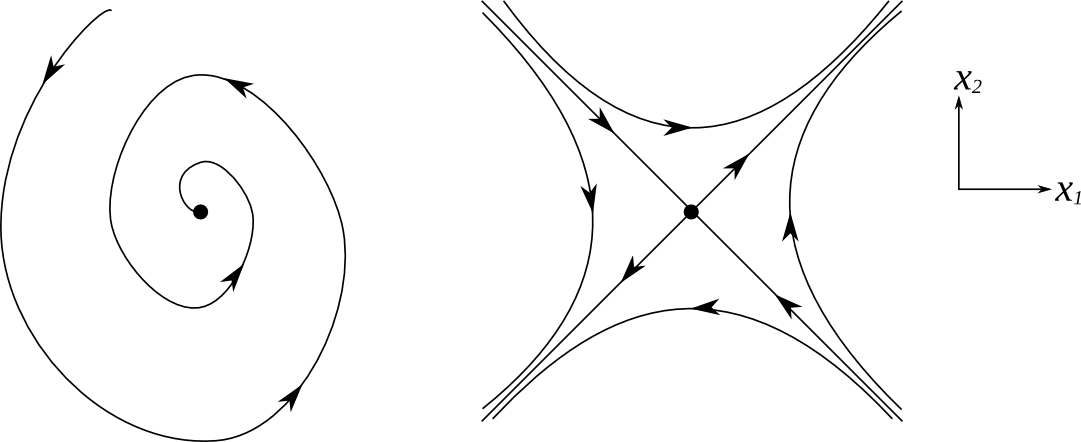
\includegraphics[width=.7\textwidth]{images/03multeq}
\caption{Local equlibria behavior.}
\label{fig:03multeq}
\end{figure}

\begin{figure}[ht!]
\centering
\includegraphics[width=.7\textwidth]{images/03globaleq}
\caption{Global equlibria behavior.}
\label{fig:03globaleq}
\end{figure}

\begin{example}
This is Example 2.5 in Khalil and explores how linearization is a good local approximation when $\text{Re} (\lambda_i)\neq0$, which are called \textit{hyperbolic equilibria}. Let the dynamics be given by
\begin{align*}
\dot{x}_1 &= -x_2 - \mu x_1(x_1^2 + x_2^2) \\
\dot{x}_2 &= x_1 - \mu x_2(x_1^2 + x_2^2)
\end{align*}
It makes sense to use polar coordinates for this example such that
\begin{align*}
x_1 &= r\cos\theta, \qquad x_2 = r\sin\theta \\
\dot{r} &= -\mu r^3, \qquad \dot{\theta} = 1
\end{align*}
Since $\dot{\theta}$ is constant the system rotates at a constant rate. The position decreases for $\mu>0$ at a cubic rate resulting in a spiral trajectory as in Figure~\ref{fig:03cubic}.

For systems with polynomial right hand side expressions we can just ignore any terms with order $n>1$ when trying to determine the Jacobian because the Taylor series expansion will ignore them. We get
$$A = \left[\begin{array}{c c} 0 & -1 \\ 1 & 0 \end{array}\right]$$
This would yield a circle. However, the nonlinear analysis shows that this is wrong and the linearization has caused this error due to the fact that $\text{Re} (\lambda_i) = 0$. Note that $\text{Re} (\lambda_{1,2}) = 0$.
$\lozenge$
\end{example}

\begin{figure}[ht!]
	\centering
	\includegraphics[width=.5\textwidth]{images/03cubic}
	\caption{Spiral trajectory.}
	\label{fig:03cubic}
\end{figure}

\section{Fundamental Properties of Nonlinear Systems}
This is Chapter 3 of Khalil and involves studying the \textit{existence} and \textit{uniqueness} of solutions of systems of the form
$$\dot{x} = f (t,x), \qquad x (t_0) = x_0$$

\begin{example}
This is a system where a solution does not exist.
\begin{align*}
\dot{x} &= -x + x^3 \\
x(t) &= \frac{x_0}{\sqrt{x_0^2(1-e^{2t}) + e^{2t}}}
\end{align*}
If $|x_0|>1$ then $|x(t)|\to\infty$ as $t\to\tfrac{1}{2}\text{ln}\frac{x_0^2}{x_0^2-1}$.
$\lozenge$
\end{example}
%%%%%%%%%%%%%%%%%%%%%%%%%%%%%%%%%%%%%%%%%%%%%%%%%%%%%%%%%%%%%
